Герон Александрийский и его эолипил (шар Герона). Принцип работы сегнерова колеса был известны задолго до 18 века. Первым задокументированным устройством была машина-игрушка, созданная Героном Александрийским. Его известное устройством представляет из себя шар. К нему из котла через две трубки подаётся пар. Эолипил может приводиться к вращению по оси, проходящей через горизонтальные участки этих труб. По оси, перпендикулярной к оси вращения, установлены изогнутые выпускные сопла. Реактивные силы истекающих струй создают вращающий момент.
Однако шар Герона оставался лабораторной установкой. Он не нашёл практического применения из-за отсутсвия эффективных способов получения пара под высоким давлением. \cite{sheypak}
\begin{center}
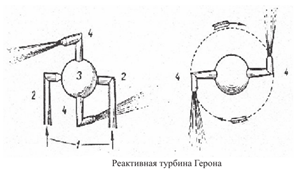
\includegraphics{Рисунок1.png}
\end{center}
Янош Андреас Сегнер(1704--1777), профессор в Гёттингенском университете, в 1750 году опубликовал работу о колесе. Он основан на вращении устройства под действием реакции вытекающей струи жидкости. Он описал случай с четырьмя трубками, изогнутыми перпендикулярно радиальному направлению, определил скорость истечения, её увеличение в зависимости от вращения, КПД. Затем Сегнер изготовил увеличенное колесо для мельницы Нёртене для привода пресса растительного масла. \cite{segner}

\begin{wrapfigure}{r}{0.25\textwidth}
    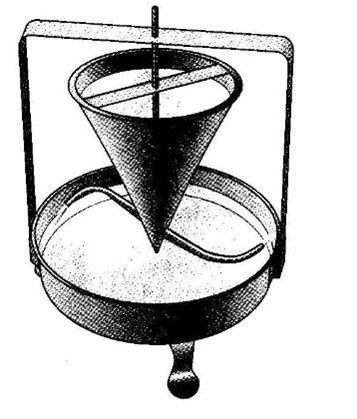
\includegraphics[width=0.27\textwidth]{Рисунок2.jpg}
\end{wrapfigure}
В отличие от шара Герона необходимость пара отсутствовала. Сегнерово колесо использовало гидростатическое давление, создаваемое разностью уровней жидкости между водоисточником и соплами. \cite{segner} Отказ от парового котла позволил создать стабильное устройство. Конструкция, предложенная Сегнером, состояла из подводящей трубы, по которой вода поступала к ротору с двумя изогнутыми соплами, направленными в противоположные стороны. Вода, вытекая из сопел, создавала реактивную силу, вызывавшую вращение ротора. Он обосновал работу устройства, установив зависимость между высотой водяного столба развиваемым моментом.

В 1754 г. Л. Эйлер привел свое мнение о быстроте и высоком КПД гидротурбины на основе колеса Сегнера. Он выполнил детальный математический анализ рабочего процесса реактивной турбины. Были созданы основы теории лопастных машин. Эксперименты показали, что КПД созданной реактивной гидротурбины при 2-метровом напоре воды составил $62,05\%$ и оказался на $5,5\%$ меньше результатов теоретических расчетов. При увеличении давления воды КПД увеличился до $74\%$. При напоре воды 2 метра и расходе воды $0,2 м^3 /с$ частота вращения гидротурбины составила 144 об/мин. Такие гидротурбины очень удобно использовать в источниках воды с низким напором 2--5 метров, из-за низкой стоимости срок окупаемости небольшой.

Рациональная идея Эйлера о конструкции гидротурбин нашла свое окончательное выражение в его предложении разделить гидравлическую машину нового типа на две части "--- неподвижную и вращающуюся. Неподвижная часть представляет собой отводящее устройство, направленный поток воды из нее поступает в нижнее вращающееся колесо, закреплённое на валу вращающегося рабочего колеса, а вода выходит оттуда через 20 изогнутых труб. Эта конструкция была переходной конструкцией от оригинальной формы колеса Сегнера к гидравлической турбине. \cite{krivchenko,bozarov2023}

В 1745 году в Лондоне вышла книга Дезагюлье, содержавшая описание водяного
двигателя, изобретённого в Англии Баркерсом, конструктивно почти идентичного сегнерову
колесу \cite{konchakov}. В историко"=технической литературе оба названия часто используются как
синонимы, однако устройство Баркерса получило более широкое распространение в
англоязычных странах, где оно было известно как <<Barker's mill>>.

В 1826 г. французский профессор Бурден (Burdin), очевидно знакомый с работами Эйлера, предложил гидравлический или водяной двигатель, впервые названный им турбиной. Латинское слово turbo, turbinus означает волчок. С тех пор этот термин применяется во многих языках. В русском языке наряду с термином лопаточная машина используется эквивалентный термин турбомашина. В двигателе Бурдена имеются два основных рабочих органа, присущих всем современным турбинам (гидравлическим, паровым, газовым), "= подвижное рабочее колесо (иногда называемый ротором турбины) и неподвижный направляющий аппарат. Вода подводится внутрь направляющего аппарата и направляется к периферии рабочего колеса, это "= центробежная машина. Бурдену не удалось найти надлежащую форму лопаток турбины, поэтому коэффициент ее полезного действия был низок.

Первая водяная турбина в России была построена на Алапаевском чугуноплавильном и железоделательном заводе. Эта турбина, мощностью в 35 л.с. сконструирована и построена плотинным мастером И. Е. Сафоновым в 1837 г. Она представляла собой чисто радиальную турбину с внутренним подводом воды. По всей вероятности, это изобретение можно считать самостоятельным достижением уральского мастера, так как описание турбины Фурнейрона на русском языке появилось только в 1839 г. в Горном журнале. На протяжении последующих пятидесяти лет в Европе и Северной Америке появилось много новых систем турбин. Больше всего на развитие гидротурбостроение оказали осевая турбина Жонваля (Jonvalle, 1843 г.), радиальная турбина Френсиса (Fransis, 1847 г.), активная тангенциальная турбина Пельтона (Pelton, Lester Allan).

На протяжении XIX-XX веков конструкция сегнерова колеса претерпела ряд изменений, направленных на повышение эффективности и расширение области применен. Основные направления эволюции включали:
\begin{enumerate}
    \renewcommand{\labelenumi}{\arabic{enumi})}
    \item увеличение числа сопел для более равномерного распределения нагрузки и снижения пульсаций момента;
    \item оптимизацию геометрии сопел (угол наклона, форма выходного сечения) для повышения скорости истечения и снижения гидравлических потерь;
    \item использование подшипников качения вместо подшипников скольжения для уменьшения механических потерь;
    \item разработку конструкций с вертикальным и горизонтальным ф вала для различных условий монтажа.
\end{enumerate}

Несмотря на эти усовершенствования, классическое сегнерово колесо сохраняло сравнительно низкий КПД - около $50\%$ \cite{konchakov}, что ограничивало его применение в промышленности, особенно на фоне развивавшихся в XIX веке более совершенных гидротурбин - радиально-осевых (турбин Френсиса) и осевых (пропеллерных). Однако простота конструкции, надёжность и способность работать на низких напорах обеспечили сохранение интереса к сегнерову колесу, особенно в сфере малой гидроэнергетики и орошения.	

